% Tamanho do texto, tipo de papel e documento
\documentclass[12pt,a4paper]{article}

% PACOTES
% Padrão
\usepackage[utf8]{inputenc}
\usepackage{amsmath}
\usepackage{amsfonts}
\usepackage{amssymb}

% Pacotes para alterar fonte
\usepackage[T1]{fontenc}
\usepackage{uarial}
% Personaliza lista de itens
\usepackage{enumitem}
% Muda fonte dos "captions"
\usepackage[font=small]{caption}
% Permite adicionar imagens
\usepackage{graphicx}
% Pacote para referências
\usepackage{csquotes}
% Coloca alguns termos do artigo em português (figura, tabela)
\usepackage[brazilian]{babel}
% Permite alterar distância entre linhas
\usepackage{setspace}
% Colocando indentação em todos os parágrafos (por default o primeiro parágrafo da seção não tem)
\usepackage{indentfirst}
% Margens nas páginas
\usepackage[top=3cm, left=3cm, bottom=2cm, right=2cm]{geometry}
% Links do sumário para as respectivas páginas
\usepackage[colorlinks=true,linkcolor=black]{hyperref}
% Visualização de códigos no meio do texto
\usepackage{listings}
% Cores no código
\usepackage{color}
% Para inserir URLs
\usepackage{hyperref}
\makeatletter
\g@addto@macro{\UrlBreaks}{\UrlOrds}
\makeatother

% CONFIGURAÇÃO DE VARIÁVEIS
% Mostra numero da pagina no canto superior direito
\pagestyle{myheadings}
% Indentação dos parágrafos
\parindent 30pt
% Distância entre linhas
\onehalfspacing
% Acessando comandos internos
\makeatletter
	% Colocando espaço de "um espaço" entre o número e o título da seção (default é espaço de 1 quad (1em))
	\renewcommand{\@seccntformat}[1]{\csname the#1\endcsname\ }
	% Deixa os itens do sumário com pontos
	\renewcommand*\l@section{\@dottedtocline{1}{1.5em}{2.3em}}
\makeatother
% Editando títulos dos índices
\addto\captionsbrazilian{
	\renewcommand{\listfigurename}{\centering LISTA DE FIGURAS}
	\renewcommand{\listtablename}{\centering LISTA DE TABELAS}
	\renewcommand{\contentsname}{\centering SUMÁRIO}
}
% Escolhendo a fonte 
\renewcommand{\familydefault}{\sfdefault}
% Estilo de listas
\renewcommand{\theenumi}{\alph{enumi}}
% Cor da URL
\hypersetup{urlcolor=black}
% Fonte da URL
\urlstyle{sf}


% INFORMAÇÕES DO TRABALHO
\author{MATEUS GONÇALEZ ETTO}
\title{UTILIZAÇÃO DE INTELIGÊNCIA ARTIFICIAL EM JOGO RPG}
\date{\today}


% COMANDOS PERSONALIZADOS
% Fonte da imagem
\newcommand{\source}[1]{\small Fonte: {#1}}
% Citações longas
\def\longcitation{\list{}{\vspace{-6mm} \leftmargin4.0cm \singlespace \small}\item[]}
\let\endlongcitation=\endlist
% Capa: objetivo do trabalho
\def\articleobjective{\list{}{\vspace{1.5cm} \leftmargin7.0cm \singlespace \small}\item[]}
\let\endarticleobjective=\endlist
% Código C#
\definecolor{codegreen}{rgb}{0,0.6,0}
\definecolor{codelightgreen}{rgb}{0.5,1,0.5}
\definecolor{codepurple}{rgb}{0.62,0,0.84}
\definecolor{codeblue}{rgb}{0,0,1}
\definecolor{backcolour}{rgb}{0.95,0.95,0.92}
\lstdefinestyle{mystyle}{
    backgroundcolor=\color{backcolour},   
    commentstyle=\color{codegreen},
    keywordstyle=\color{codeblue},
    numberstyle=\tiny\color{codelightgreen},
    stringstyle=\color{codepurple},
    basicstyle=\footnotesize,
    breakatwhitespace=false,
    breaklines=true,
    captionpos=b,
    keepspaces=true,
    numbers=left,
    numbersep=5pt,
    showspaces=false,
    showstringspaces=false,
    showtabs=false,
    tabsize=2
}
\lstset{literate=
  {á}{{\'a}}1 {é}{{\'e}}1 {í}{{\'i}}1 {ó}{{\'o}}1 {ú}{{\'u}}1
  {Á}{{\'A}}1 {É}{{\'E}}1 {Í}{{\'I}}1 {Ó}{{\'O}}1 {Ú}{{\'U}}1
  {à}{{\`a}}1 {è}{{\`e}}1 {ì}{{\`i}}1 {ò}{{\`o}}1 {ù}{{\`u}}1
  {À}{{\`A}}1 {È}{{\'E}}1 {Ì}{{\`I}}1 {Ò}{{\`O}}1 {Ù}{{\`U}}1
  {ä}{{\"a}}1 {ë}{{\"e}}1 {ï}{{\"i}}1 {ö}{{\"o}}1 {ü}{{\"u}}1
  {Ä}{{\"A}}1 {Ë}{{\"E}}1 {Ï}{{\"I}}1 {Ö}{{\"O}}1 {Ü}{{\"U}}1
  {â}{{\^a}}1 {ê}{{\^e}}1 {î}{{\^i}}1 {ô}{{\^o}}1 {û}{{\^u}}1
  {Â}{{\^A}}1 {Ê}{{\^E}}1 {Î}{{\^I}}1 {Ô}{{\^O}}1 {Û}{{\^U}}1
  {œ}{{\oe}}1 {Œ}{{\OE}}1 {æ}{{\ae}}1 {Æ}{{\AE}}1 {ß}{{\ss}}1
  {ű}{{\H{u}}}1 {Ű}{{\H{U}}}1 {ő}{{\H{o}}}1 {Ő}{{\H{O}}}1
  {ç}{{\c c}}1 {Ç}{{\c C}}1 {ø}{{\o}}1 {å}{{\r a}}1 {Å}{{\r A}}1
  {€}{{\EUR}}1 {£}{{\pounds}}1
}
\lstset{style=mystyle}


% INICIO DO ARTIGO
\begin{document}

% CAPA - INÍCIO
\thispagestyle{empty} % Oculta o número da página
\begin{center}
\makeatletter
	\textbf{UNIVERSIDADE ESTADUAL PAULISTA}\\
	\textbf{FACULDADE DE CIÊNCIAS}\\
	\textbf{DEPARTAMENTO DE COMPUTAÇÃO}\\
	\textbf{BACHARELADO EM CIÊNCIA DA COMPUTAÇÃO}\\

	\vspace{4.5cm} % Adicionando espaço extra
	\textbf{\@author}

	\vspace{4.5cm} % Adicionando espaço extra
	\textbf{\large \@title}
	
	\vspace*{\fill} % Adicionando espaço para escrever em baixo
	BAURU – SP\\
	\the\year
\makeatother
\end{center}
% CAPA - FIM

% FOLHA DE ROSTO - INÍCIO
\newpage % Coloca o conteúdo numa nova página
\thispagestyle{empty} % Oculta o número da página
\begin{center}
\makeatletter
	\textbf{\@author}

	\vspace{4.5cm} % Adicionando espaço extra
	\textbf{\large \@title}
\makeatother
\end{center}

\begin{articleobjective}
	Trabalho de Conclusão de Curso de graduação apresentado à disciplina Projeto e Implementação de Sistemas do curso de Bacharelado em Ciência da Computação da Faculdade de Ciências da Universidade Estadual Paulista "Júlio de Mesquita Filho"{} como requisito para obtenção do título de Bacharel em Ciência da Computação.
	
	\vspace{1.0cm} % Adicionando espaço extra
	Orientadora: Profa. Dra. Simone das Graças Domingues Prado
\end{articleobjective}

\begin{center}
	\vspace*{\fill} % Adicionando espaço para escrever em baixo
	BAURU – SP\\
	\the\year
\end{center}
% FOLHA DE ROSTO - FIM

% FOLHA DE APROVAÇÃO - INÍCIO
\newpage % Coloca o conteúdo numa nova página
\thispagestyle{empty} % Oculta o número da página
\begin{center}
\makeatletter
	\textbf{\@author}

	\vspace{3.0cm} % Adicionando espaço extra
	\textbf{\large \@title}
\makeatother
\end{center}

\begin{articleobjective}
	Trabalho de Conclusão de Curso de graduação apresentado à disciplina Projeto e Implementação de Sistemas do curso de Bacharelado em Ciência da Computação da Faculdade de Ciências da Universidade Estadual Paulista "Júlio de Mesquita Filho"{} como requisito para obtenção do título de Bacharel em Ciência da Computação.
\end{articleobjective}

\begin{center}
	\vspace{1.0cm}
	BANCA EXAMINADORA\\
	
	\vspace{1.0cm}
	\underline{\hspace{8cm}}\\
	Profa. Dra. Simone das Graças Domingues Prado\\
	\vspace{1.0cm}
	\underline{\hspace{8cm}}\\
	(Nome do segundo membro da Banca Examinadora)\\
	\vspace{1.0cm}
	\underline{\hspace{8cm}}\\
	(Nome do terceiro membro da Banca Examinadora)

	\vspace*{\fill} % Adicionando espaço para escrever em baixo
	Bauru, \underline{\hspace{1cm}} de \underline{\hspace{3cm}} de \underline{\hspace{1.5cm}}
\end{center}
% FOLHA DE APROVAÇÃO - FIM

% RESUMO - INÍCIO
\newpage % Coloca o conteúdo numa nova página
\thispagestyle{empty} % Oculta o número da página
\section*{\hfil RESUMO} % \hfil centraliza o título
	\singlespace
	\noindent
	Este projeto trata-se da criação de um protótipo de jogo no estilo RPG em turnos,
	em conjunto com a criação de uma Inteligência Artificial capaz de controlar os personagens,
	assim como de aprender a controlá-los melhor com treinamento.
	Para a criação da Inteligência Artificial,
	foram usados conceitos de Redes Neurais Artificiais e Algorítimo Genético,
	e para a criação do jogo e seus scripts
	foi usado o motor de jogo Unity.
	
	\vspace{0.8cm}
	\noindent
	\textbf{PALAVRAS-CHAVE:} Inteligência Artificial, Unity, jogo RPG
% RESUMO - FIM

\onehalfspacing

% ABSTRACT - INÍCIO
\newpage % Coloca o conteúdo numa nova página
\thispagestyle{empty} % Oculta o número da página
\section*{\hfil ABSTRACT} % \hfil centraliza o título
	\singlespace
	\noindent
	This project comes to creating a turn-based RPG game prototype,
	in conjunction with an Artificial Intelligence that is able to control the characters
	as well as to learn how to control them better with training.
	For the creation of the Artificial Intelligence,
	concepts of Artificial Neural Networks and Genetic Algorithm were used,
	and for the creation of the game and its scripts,
	the Unity game engine was used.
	
	\vspace{0.8cm}
	\noindent
	\textbf{KEY-WORDS:} Artificial Intelligence, Unity, RPG game
% ABSTRACT - FIM

\onehalfspacing

% LISTA DE FIGURAS - INÍCIO
\newpage % Coloca o conteúdo numa nova página
\thispagestyle{empty} % Oculta o número da página
\listoffigures % Cria a lista de figuras
% LISTA DE FIGURAS - FIM

% LISTA DE TABELAS - INÍCIO
\newpage % Coloca o conteúdo numa nova página
\thispagestyle{empty} % Oculta o número da página
\listoftables % Cria a lista de tabelas
% LISTA DE TABELAS - FIM

% SUMÁRIO - INÍCIO
\newpage % Coloca o conteúdo numa nova página
\thispagestyle{empty} % Oculta o número da página
\tableofcontents % Cria o Sumário
% SUMÁRIO - FIM

% INTRODUÇÃO - INÍCIO
\newpage % Coloca o conteúdo numa nova página
\section{INTRODUÇÃO}
	Há ainda muitas pessoas que acreditam que jogos eletrônicos são para crianças ou pessoas desocupadas.
	Talvez isso fosse verdade no milênio passado, mas a realidade vem se mostrando ser bem diferente.
	
	De acordo com uma pesquisa da SuperData,
	o mercado de jogos cresceu 8\% de 2014 a 2015,
	com 61 bilhões de dólares circulando nesta indústria (CNBC, 2016).
	Em 2014, o valor da indústria de jogos já havia ultrapassado o da indústria de música em 20 bilhões,
	e está chegando ao da indústria do filmes (NYTIMES, 2014).
	
	Então é fato, a indústria de jogos está movendo bilhões de dólares pelo mundo,
	já passou do de música e não para de crescer.
	Como diz o gerente de produto da Eletronic Sports League, James Lampkin:
	%no artigo da New York Times:
	"Isto está se expandindo fora de controle"{}
	(NYTIMES, 2014, tradução nossa).
	Tais palavras explicam muito bem o estado atual do mercado de jogos.
	
	E não é só nas vendas de jogos e consoles,
	existem muitos torneios de jogos ocorrendo pelo mundo,
	surgindo uma nova categoria de profissionais que,
	em poucos anos atrás era inimaginável, senão motivo de piada,
	que é a categoria de jogador profissional de jogo eletrônico.
	A área de trabalho já existe e é chamada de Esporte Eletrônico (NYTIMES, 2014).
	
	E mesmo nestes torneios, não é por pouco dinheiro que os jogadores se enfrentam.
	No Campeonato Mundial de 2015 (o quinto da série) de League of Legends,
	foi oferecido 1 milhão de dólares para a equipe vencedora mundial do jogo,
	como pode ser visto nas regras do campeonato\footnote{Regras: \url{https://riot-web-static.s3.amazonaws.com/lolesports/Rule\%20Sets/2015\%20Revised\%20World\%20Championship\%20Rule\%20Set\%20Version\%201\_01.pdf}}.
	
	Os prêmios não param por aí.
	O jogo Dota 2 distribuiu 11 milhões de dólares para os 10 melhores do mundo,
	sendo 5 milhões para os campeões,
	se tornando assim o maior prêmio já oferecido em um torneio de jogo eletrônico (NYTIMES, 2014).
	
	E tem muita gente para assistir a estes campeonatos.
	Nos dados mostrados pela Riot\footnote{Dados disponíveis em: \url{http://www.lolesports.com/en_US/articles/worlds-2015-viewership}}
	sobre o Campeonato Mundial de 2015,
	houveram 334 milhões de telespectadores "únicos"{} durante as 4 semanas do torneio,
	somando 360 milhões de horas de visualizações das partidas ao vivo.
	
	Mas a área de jogos não está chamando apenas a atenção do mercado,
	mas também a de pesquisadores.
	Um exemplo é o desenvolvimento e aplicação de técnicas de Inteligência Artificial (IA) em jogos,
	que de acordo com especialistas,
	existem áreas dentro de IA em jogos que ainda estão inexplorados (YANNAKAKIS; TOGELIUS, 2014).
	
	Em 2007, foi montada pela AiGameDev uma lista dos 10 jogos com Inteligência Artificial mais influentes.
	Um exemplo é um jogo chamado Creatures,
	que implementou aprendizado de máquina em uma simulação interativa
	ao usar Redes Neurais nas criaturas do jogo.
	Outro exemplo é o Halo,
	o jogo que implementou pela primeira vez a "árvore de condutas",
	tecnologia que ficou muito popular na indústria de jogos (AIGAMEDEV, 2007).
	
	Um exemplo de IA em jogo que é descrito em detalhes é o F.E.A.R.,
	um jogo FPS em primeira pessoa
	que criou um sistema dinâmico, coordenado, interessante e desafiador.
	Isto foi feito utilizando um sistema chamado Goal Oriented Action Planning (Planejamento de Ações Orientado a Objetivo),
	que foi construído junto de duas técnicas: Algoritmo A* e Máquina de Estados Finitos.
	Os NPCs possuem uma lista de objetivos,
	então durante o jogo eles buscam o plano que irá completar o objetivo com maior prioridade.
	O planejamento feito é similar ao STRIPS,
	tendo-se a situação atual e quais são as ações necessárias para cumprir o objetivo.
	Além disto, foi implementado uma extensão da conduta individual dos NPCs,
	com uma conduta em equipe.
	No entanto, como a conduta dos NPCs foi criada para minimizar a ameaça a si mesmo,
	os extintos básicos do NPC podem sobrescrever a conduta de equipe
	caso a segunda opção seja muito arriscado para si mesmo (ORKIN, 2006).
	
	Percebe-se, desta forma, que a área de jogos está muito ativa e em pleno crescimento,
	tanto no mercado quando em pesquisas.
	Existem áreas inexploradas de IA em jogos,
	com novas fronteiras a serem exploradas.
	Com isto em mente, este trabalho foi desenvolvido,
	%aumentando o número de trabalhos que estão explorando esta área,
	e espera-se contribuir com a comunidade acadêmica e/ou mercado de alguma forma.

	\subsection{Objetivos do Trabalho}
	
		\subsubsection{Objetivo Geral}
			Produzir um jogo RPG em turnos que implementa conceitos avançados de Inteligência Artificial,
			sendo esta inteligência capaz de tomar decisões de forma autônoma sobre o que deve fazer,
			assim como ser capaz de aprender a tomar melhores decisões por meio de treinamento.
		
		\subsubsection{Objetivos Específicos}
			\begin{enumerate}[noitemsep]
				\item Criar um jogo RPG razoavelmente complexo.
				\item Criar uma Inteligência Artificial capaz de jogar o jogo tão bem quanto um ser humano.
				\item Criar uma Inteligência Artificial capaz de aprender conforme joga.
			\end{enumerate}			
	
	\subsection{Organização da Monografia}
		Este trabalho está dividido em 5 seções, sendo esta seção (Introdução) a primeira. As outras seções são:
		\begin{itemize}[noitemsep]
     		\item Seção 2, \textbf{Ferramentas Utilizadas:} apresentação das ferramentas utilizadas para o desenvolvimento do projeto proposto no trabalho.
     		\item Seção 3, \textbf{Conceitos:} explicação das teorias de Inteligência Artificial e Algoritmo Genético usadas para desenvolver o trabalho.
     		\item Seção 4, \textbf{O Jogo:} descrição em detalhes do jogo, suas variáveis, e de sua implementação.
     		\item Seção 5, \textbf{Resultados:} apresentação dos resultados obtidos no trabalho.
  	 	\end{itemize}
% INTRODUÇÃO - FIM

% DESENVOLVIMENTO - INÍCIO
\newpage % Coloca o conteúdo numa nova página
\section{FERRAMENTAS UTILIZADAS}

	\subsection{Unity}
		A Unity é um motor de jogo multiplataforma que permite a criação de jogos 2D ou 3D.
		Possui uma interface gráfica que permite desenvolver jogos com facilidade,
		além de ter muitos serviços integrados que aceleram o processo de desenvolvimento.
		As linguagens de programação que podem ser usadas são UnityScript e C\#
		(UNITY, 2016a).
		
		Com mais de 200 jogos na lista de jogos em destaque que foram criados na Unity,
		um dos exemplos que pode-se citar é o \textit{Sky Force},
		um jogo no estilo de ação, missões e "shooter",
		e que está disponível na App Store e Google Play.
		Outro exemplo é o \textit{The Uncertain},
		do qual o jogador é um robô e
		deve resolver quebra-cabeças em uma aventura.
		O jogo está disponível na \textit{Steam}
		(UNITY, 2016b).
		
		O editor da Unity também é extensível, sendo possível implementar funcionalidades ainda não existentes
		(UNITY, 2016a).
		Um exemplo de extensão é o \textit{Rival Theory},
		que implementa vários conceitos de Inteligência Artificial,
		desde funcionalidades básicas como \textit{pathfinding},
		condutas de patrulha, esconder, atacar, seguir, vaguear,
		até conceitos mais complicados como percepção e árvore de condutas
		(RIVAL THEORY, 2015).
		
		\subsubsection{Interface}
			A interface da Unity é composta por vários painéis chamados \textit{views},
			que podem ser rearranjados, agrupados, separados e fixados
			(UNITY, 2016c).
			O arranjamento padrão das janelas permite o acesso às janelas mais comuns,
			e pode ser visto na figura a seguir:
			
			\begin{figure}[ht!]
				\label{interfaceUnity}
				\caption{A interface padrão da Unity}
				\centering
				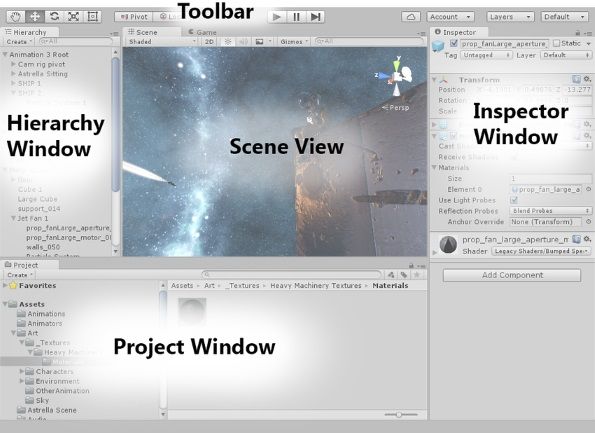
\includegraphics[scale=0.5]{InterfaceUnity.jpg}\\
				\vspace{0.5mm}
				\source{Unity.}
			\end{figure}	
			
			A descrição de cada painel pode ser vista na tabela a seguir:
			
			\begin{table}[ht]
				\label{tabelaUnity}
				\caption{Descrição dos painéis na Unity}
				\centering
				\small
				\begin{tabular}{p{3.1cm} p{11.9cm}}
					\hline 
					Project Window & Exibe a biblioteca de Assets que estão disponíveis para uso no projeto. Ao importar os Assets no projeto, eles aparecerão aqui. \\ 
					\hline 
					Scene View & Permite navegar visualmente e editar a cena. A Scene View pode mostrar em perspectiva 3D ou 2D, dependendo do tipo de projeto que está sendo trabalhando. \\ 
					\hline 
					Hierarchy Window & É uma representação de texto hierárquica de cada objeto na cena. Cada item na cena tem uma entrada na hierarquia, de forma que as duas janelas estão inerentemente conectadas. A hierarquia revela a estrutura da forma como os objectos estão ligados um ao outro. \\ 
					\hline 
					Inspector Window & Permite visualizar e editar todas as propriedades do objeto selecionado. Como diferentes tipos de objetos têm diferentes conjuntos de propriedades, o layout e conteúdo da janela do Inspector pode variar. \\ 
					\hline 
					Toolbar & Fornece acesso aos recursos de trabalho mais essenciais. À esquerda estão as ferramentas básicas para manipular a Scene View e os objetos dentro dela. No centro estão os controles de play, pause e step. Os botões à direita dará acesso aos Serviços da Unity Cloud e da Conta Unity, seguido pelo menu de visibilidade dos layers e, finalmente, o menu de layout do editor (que fornece alguns layouts alternativos para as janelas do editor, e permite salvar um layout customizado). \\ 
					\hline 
				\end{tabular}\\
				\vspace{3mm}
				\source{Unity.}
			\end{table}
			
			Os objetos contidos na cena do projeto são chamados de \textit{GameObject},
			sendo que suas características podem ser alteradas por Componentes anexados a ele.
			A Unity possui vários Componentes prontos,
			no entanto é possível criar novos usando as linguagens de programação do qual se dá suporte (C\# e UnityScript).
			Tais Componentes são chamados de Scripts,
			e eles permitem disparar eventos,
			modificar as propriedades de outros Componentes ou do próprio \textit{GameObject} durante o jogo,
			e a interação com o jogador.
			(UNITY, 2016d).

	\subsection{Visual Studio}
		O Visual Studio é um Ambiente de Desenvolvimento Integrado (IDE) usado para a criação de aplicativos para Windows, Android, iOS, aplicações Web e serviços de nuvem.
		Com ele é possível programar em C\#, Visual Basic, F\#, C++, HTML, JavaScript e Python, dentre outras linguagens de programação. (MICROSOFT, 2016)
		
		A integração do Visual Studio com a Unity, usando C\#, ocorre com a adição do \textit{namespace} UnityEngine ao script,
		%(com o código "using UnityEngine"),
		liberando a utilização da classe \textit{MonoBehaviour},
		da qual possui implementado funcionalidades e funções internas da Unity.
		Para utilizar a classe \textit{MonoBehaviour} nos scripts criados,
		basta estender a classe criada com a \textit{MonoBehaviour} (UNITY, 2016d).
		Desta forma, o cabeçalho do script fica como no código a seguir:
		
		\begin{lstlisting}[language=C++]
using UnityEngine;

public class nomeDaClasse : MonoBehaviour
{
	// Código da classe
}\end{lstlisting}
		
		Com isto feito, é possível utilizar uma das principais vantagens do Visual Studio,
		que é o \textit{AutoComplete}.
		Ou seja, funções internas da Unity, como as do GameObject, aparecem em uma lista conforme se vai digitando,
		facilitando muito a programação do script.
		
		Além da integração com a Unity,
		ainda é possível utilizar as bibliotecas próprias do C\#,
		como bibliotecas matemáticas, acesso à arquivo e listas.
		
		Na \textit{Figura \ref{fig:exvs}} a seguir, é possível ver um exemplo de classe criada no Visual Studio que foi usada neste projeto:
		
		\begin{figure}[ht!]
			\caption{Exemplo de classe no Visual Studio}
			\centering
			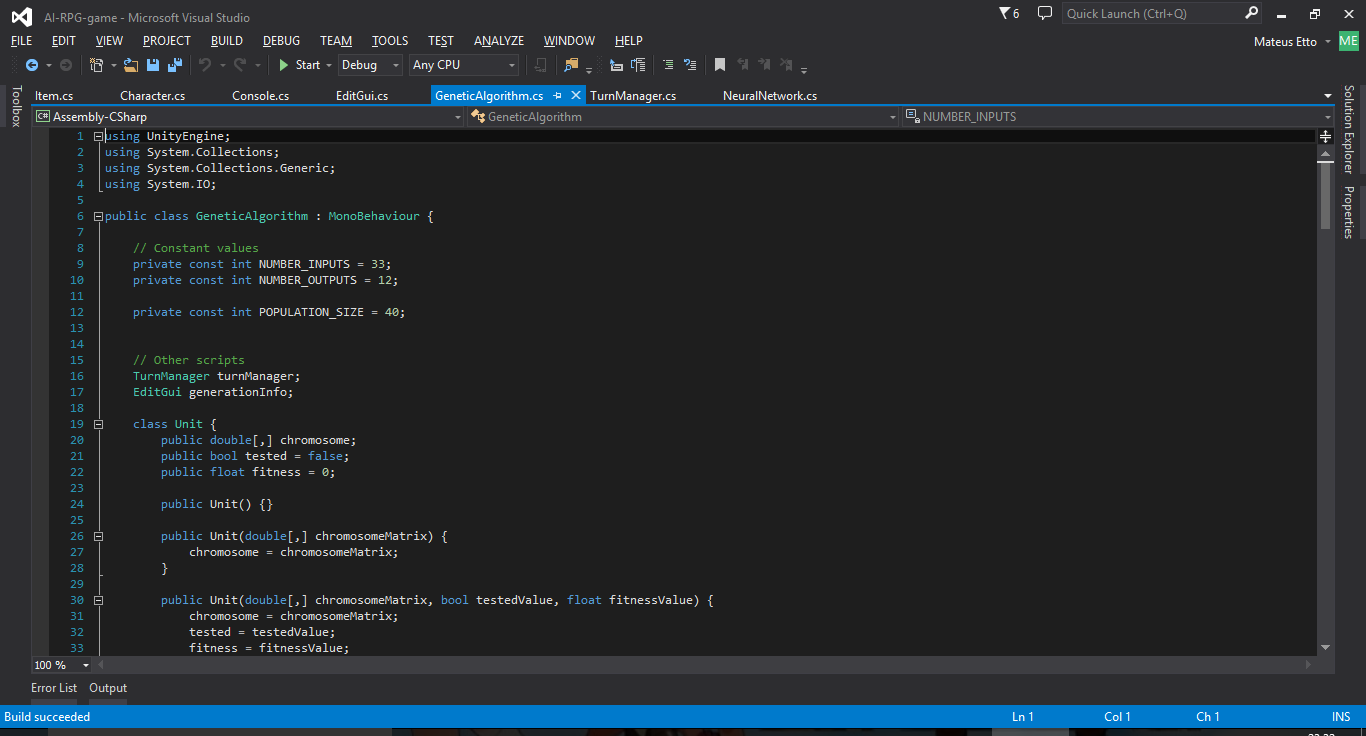
\includegraphics[scale=0.4]{InterfaceVisualStudio.png}\\
			\vspace{0.5mm}
			\source{Elaborado pelo autor.}
			\label{fig:exvs}
		\end{figure}
		
		Note que no script de Algoritmo Genético, além do \textit{UnityEngine} e outras duas bibliotecas básicas do C\#,
		também foi utilizada o \textit{System.IO}, uma biblioteca para Leitura e Escrita de Arquivo.
		Qualquer outro script criado para funcionar na Unity tem este padrão.

\newpage % Coloca o conteúdo numa nova página	
\section{CONCEITOS}

	Nesta seção será descrito dois conceitos que foram amplamente utilizados neste trabalho,
	que são Redes Neurais Artificiais (RNA) e Algoritmo Genético (AG).
	Apesar de ser possível descrever várias variações de aplicação desses conceitos,
	será explicado apenas a essência deles,
	e o que foi necessário para desenvolver este trabalho.

	\subsection{Redes Neurais}
	As Redes Neurais Artificiais foram inspiradas no funcionamento do cérebro humano,
	e a "baixo nível"{} procura imitar o que acontece nos neurônios.
	
	Uma RNA é normalmente utilizada para duas finalidades:
	reconhecimento de padrões e regressão (ou aproximação de função).
	A arquitetura de uma RNA é formada por uma camada de entrada (input layer),
	uma camada de saída (output layer),
	e as camadas ocultas (hidden layers),
	que podem ter de zero a muitas camadas.
	
	Um exemplo de Rede Neural Artificial com uma camada oculta pode ser visto na Figura \ref{fig:basicnn} a seguir:
	
	\begin{figure}[ht!]
		\caption{RNA com uma camada oculta}
		\centering
		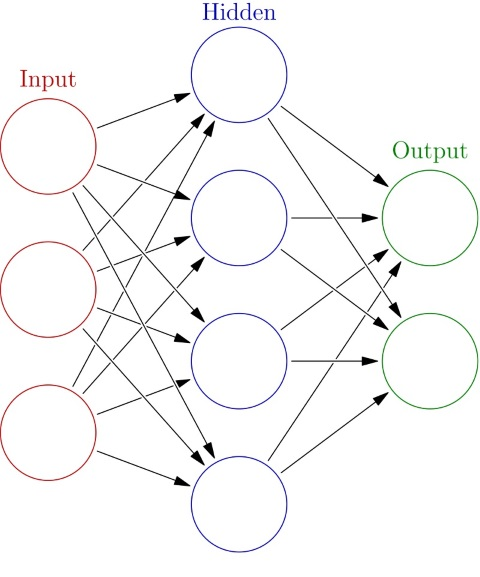
\includegraphics[scale=0.5]{BasicNN.jpg}\\
		\vspace{0.5mm}
		\source{Wikimedia.}
		\label{fig:basicnn}
	\end{figure}
	
	Uma Rede Neural Artificial sempre terá uma camada de entrada e uma de saída.
	No entanto, o número de camadas ocultas pode variar bastante entre um problema e outro,
	assim como o número de neurônios contidos nessas camadas.
	Estas camadas ocultas são explicadas como sendo "extratoras de características"{}
	(STACKEXCHANGE, 2013).
	
	Como o número de camadas ocultas é escolhido?
	Caso os dados sejam linearmente separáveis,
	não é necessário nenhuma camada oculta.
	Existem muitas discussões a respeito do número de camadas ocultas a serem usadas, caso ela seja necessária,
	mas um consenso que existe é que uma camada é suficiente para a maioria dos problemas
	(STACKEXCHANGE, 2013).
	
	\begin{figure}[ht!]
		\caption{Importância de ter camada oculta}
		\centering
		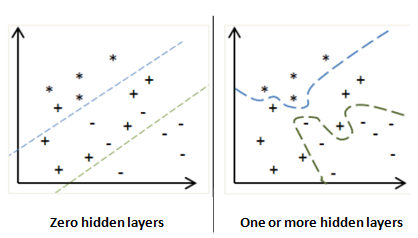
\includegraphics[scale=1.5]{HiddenLayers.png}\\
		\vspace{0.5mm}
		\source{Stackoverflow.}
		\label{fig:nnhiddenlayer}
	\end{figure}
	
	Como pode-se notar na Figura \ref{fig:nnhiddenlayer},
	o aumento de camadas ocultas aumenta a granularidade do reconhecimento de padrões,
	fazendo-se assim uma separação não-linear no reconhecimento dos dados de entrada.
	
	Para descobrir o número de neurônios a serem colocados na camada oculta
	existem muitas regras empíricas que ajudam a escolher um valor,
	mas uma delas que funciona com frequência é encontrar a média do número de neurônios de entrada e de saída.
	Usa-se este valor empírico como valor inicial para número de neurônios na camada oculta,
	e então ajusta-se este valor com testes
	(STACKEXCHANGE, 2013).
	
	A escolha da função de saída dos neurônios também tem bastante influência na convergência da Rede Neural.
	De maneira geral pode-se separar que tipo de função a ser utilizada dependendo da tarefa:
	reconhecimento de padrões ou regressão de uma função
	(RESEARCHGATE, 2013).
	
	Caso a tarefa seja de reconhecer padrões,
	as funções recomendadas são a step, sigmóide e tangente hiperbólica.
	O motivo é que estas funções retornam valores entre um intervalo pré-estabelecido.
	(RESEARCHGATE, 2013).
	
	Por outro lado, caso a tarefa seja de regressão de uma função,
	pode-se utilizar a função linear na camada de saída.
	No entanto, nas camadas ocultas ainda é necessário o uso de funções não lineares.
	Caso as camadas ocultas também sejam de função linear,
	as soluções a serem encontradas serão apenas linearmente separáveis,
	equivalente a uma rede sem camada oculta
	(RESEARCHGATE).

	\subsection{Algoritmo Genético}
	Algoritmo genético faz parte da computação evolutiva,
	e baseia-se na teoria de Darwin sobre a evolução das espécies.
	
	O algoritmo inicia com um conjunto de soluções,
	e eles são representados por cromossomos.
	Este conjunto é a população, e aqueles que conseguirem se adaptar melhor,
	passarão para a próxima geração.
	A motivação do AG é que as soluções melhoram a cada geração.
	
	De maneira geral, um Algoritmo Genético segue o seguinte processo:
	
	\begin{itemize}[noitemsep]
		\item \textbf{Iniciar População:} Gera uma população aleatória de n cromossomos.
		\item \textbf{Teste:} Testa o valor de fitness f(x) de cada cromossomo x da população.
		Se a condição de parada for satisfeita, o algoritmo acaba.
		\item \textbf{Seleção:} Seleciona 2 cromossomos de acordo com o fitness deles,
		ou seja, quanto maior o valor de fitness, maior a probabilidade.
		Normalmente é utilizado o método da roleta para a seleção.
		\item \textbf{Crossover:} Copia partes dos cromossomos dos pais em cromossomos filhos,
		aplicando uma determinada probabilidade de alternar o trecho a ser copiado.
		\item \textbf{Mutação:} Probabilidade de algum valor do cromossomo do novo filho ser alterado.
		\item \textbf{Inserção:} Insere os novos cromossomos na população.
		\item \textbf{Loop:} Retorna ao passo de calcular o "fitness".
	\end{itemize}
	
	No trabalho aqui desenvolvido,
	Redes Neurais Artificiais e Algoritmos Genéticos são utilizados juntos.
	O cromossomo do Algorítmo Genético se torna, neste caso, os pesos que estão nos neurônios da RNA.
	Desta forma, o AG estará procurando as soluções ótimas da Rede Neural.

\newpage % Coloca o conteúdo numa nova página
\section{O JOGO}
	
	\subsection{Descrição do jogo}
	<Descrever o jogo, suas variáveis, complexidades, particularidades, etc>
	
	\subsection{Rede Neural Artificial Implementado}
	<Descrever em detalhes qual foi a Rede Neural Artificial implementada>
	
	\subsection{Algoritmo Genético Implementado}
	<Descrever em detalhes qual foi o Algoritmo Genético implementado>
	
	\subsection{Funcionamento do jogo}
	<Descrever como ocorre o funcionamento do jogo como um todo, dado que o leitor sabe os detalhes de cada parte.>

% DESENVOLVIMENTO - FIM

% CONCLUSÃO - INÍCIO
\newpage % Coloca o conteúdo numa nova página
\section{RESULTADOS}
	<Inserir gráficos de evolução do algoritmo, imagens do jogo, explicar desempenho da aprendizagem, etc.>
% CONCLUSÃO - FIM

\newpage % Coloca o conteúdo numa nova página
\section*{REFERÊNCIAS}
\addcontentsline{toc}{section}{REFERÊNCIAS} % Adiciona as referências no Sumário
	\singlespace
	UNITY. Game engine, tools and multiplatform. 2016a. Disponível em: \textless \url{https://unity3d.com/pt/unity}\textgreater. Acesso em 01 Julho 2016.\par
	UNITY. Made with Unity - Games. 2016b. Disponível em: \textless \url{https://madewith.unity.com/games}\textgreater. Acesso em 01 Julho 2016.\par
	UNITY. Made with Unity - Manual: Learning the Interface. 2016c. Disponível em: \textless \url{https://docs.unity3d.com/Manual/LearningtheInterface.html}\textgreater. Acesso em 05 Julho 2016.\par
	UNITY. Made with Unity - Manual: Creating and Using Scripts. 2016d. Disponível em: \textless \url{https://docs.unity3d.com/Manual/CreatingAndUsingScripts.html}\textgreater. Acesso em 05 Julho 2016.\par
	RIVAL THEORY. Features. 2015. Disponível em: \textless \url{http://rivaltheory.com/rain/features/}\textgreater. Acesso em 01 Julho 2016.\par
	MICROSOFT. Free Dev Tools - Visual Studio Community 2015. 2016. Disponível em: \textless \url{https://www.visualstudio.com/en-us/products/visual-studio-community-vs.aspx}\textgreater. Acesso em 07 Julho 2016.\par
	CNBC. Digital gaming sales hit record \$61 billion in 2015: Report. Disponível em: \textless \url{http://www.cnbc.com/2016/01/26/digital-gaming-sales-hit-record-61-billion-in-2015-report.html}\textgreater. Acesso em 11 Julho 2016.\par
	YANNAKAKIS, Georgios N; TOGELIUS, Julian. A Panorama of Artificial and Computational Intelligence in Games. Disponível em: \textless \url{http://julian.togelius.com/Yannakakis2014Panorama.pdf}\textgreater. Acesso em 11 Julho 2016.\par
	AIGAMEDEV. Top 10 Most Influential AI Games. Disponível em: \textless \url{http://aigamedev.com/open/highlights/top-ai-games/}\textgreater. Acesso em 12 Julho 2016.\par
	ORKIN, Jeff. Three States and a Plan: The A.I. of F.E.A.R. Disponível em: \textless \url{http://alumni.media.mit.edu/~jorkin/gdc2006_orkin_jeff_fear.pdf}\textgreater. Acesso em 12 Julho 2016.\par
	STACKEXCHANGE. How to choose the number of hidden layers and nodes in a feedforward neural network?. Disponível em: \textless \url{https://stats.stackexchange.com/questions/181/how-to-choose-the-number-of-hidden-layers-and-nodes-in-a-feedforward-neural-netw}\textgreater. Acesso em 13 Julho 2016.\par
	STACKEXCHANGE. What does the hidden layer in a neural network compute?. Disponível em: \textless \url{https://stats.stackexchange.com/questions/63152/what-does-the-hidden-layer-in-a-neural-network-compute}\textgreater. Acesso em 13 Julho 2016.\par
	STACKOVERFLOW. Role of Bias in Neural Networks. Disponível em: \textless \url{https://stackoverflow.com/questions/2480650/role-of-bias-in-neural-networks}\textgreater. Acesso em 13 Julho 2016.\par
	OBITKO, Marek. Introduction to Genetic Algorithms. Disponível em: \textless \url{http://www.obitko.com/tutorials/genetic-algorithms/index.php}\textgreater. Acesso em 13 Julho 2016.\par
	RESEARCHGATE. How to select the best transfer function for a neural network model?. Disponível em: \textless \url{https://www.researchgate.net/post/How_to_select_the_best_transfer_function_for_a_neural_network_model}\textgreater. Acesso em 13 Julho 2016.\par
	Wikimedia. File:Colored neural network.svg. Disponível em: \textless \url{https://commons.wikimedia.org/wiki/File:Colored_neural_network.svg}\textgreater. Acesso em 13 Julho 2016.\par
	STACKOVERFLOW. How do you decide the parameters of a Convolutional Neural Network for image classification?. Disponível em: \textless \url{https://stackoverflow.com/questions/24509921/how-do-you-decide-the-parameters-of-a-convolutional-neural-network-for-image-cla}\textgreater. Acesso em 13 Julho 2016.\par

\end{document}
